
\chapter{Methodology} \label{cap:metodos}


% ISSO aqui é metodologia
%Como foi evidenciado nas comunicações com a gestão do restaurante, a análise utilizada para se prever as refeições é produzir no dia da semana, como por exemplo uma segunda-feira, o consumo do mesmo dia da semana anterior (segunda-feira anterior) com acréscimo de uma margem de erro. Em geral, de acordo com o restaurante, todos os dias o mesmo trabalha com um erro e um descarte de 30\% das refeições que são trazidas e consumidas ao campus. Estima-se então que no período de 2011 - 01/08/2018 os estabelecimentos tenham tido um prejuízo de R\$1.885.938,40, e de 30\% de R\$78.386,85 no atual período de 01/08/2018 - 31/10/2018 totalizando o montante  R\$1.964.325,25. Aproximadamente 2 milhões de reais em prejuízo acumulado desde 2011.



% A obtenção dos dados do R.U do ICT Unifesp se encontra em formato de série temporal, ou seja, o consumo e vendas de refeições no R.U se distribuem em função do tempo, pelos dias letivos da universidade.
 
 
 % O cenário deste estudo analisa a sazonalidade da frequência de alunos do ICT - UNIFESP, inferida pelas grades semestrais de suas disciplinas, que consequentemente inferem na sazonalidade de consumo de refeições dentro do restaurante universitário. 
 
 
 
 
   This chapter describes the experimental methodology of this study, which consists of the following steps:
    \begin{itemize}
        \item Collection of endogenous and exogenous data.
        \item Transformation of each endogenous data record (the consumption and sales data), into a time series with an interval of previous five days.
        \item Exploratory analysis of endogenous and exogenous data sets with the data set to be predicted.
        \item Construction and training of exclusively endogenous and mixed models, duplicated in two experimental phases with different time domains.
        \item Comparative analysis of the model results.
    \end{itemize}
    
    \section{Field of Study}
       The field of study of this project is the university refectory of the Science and Technology Institute of Unifesp (ICT-Unifesp) in São José dos Campos. The ICT campus was inaugurated in 2007 aiming to supply the scientific and technological demands of the Vale do Paraíba region. The Figure \ref{fig:RU_foto} presents a common day of use of the physical space of the university refectory in ICT.
        
        \begin{figure}[H]
        	\center{
        	    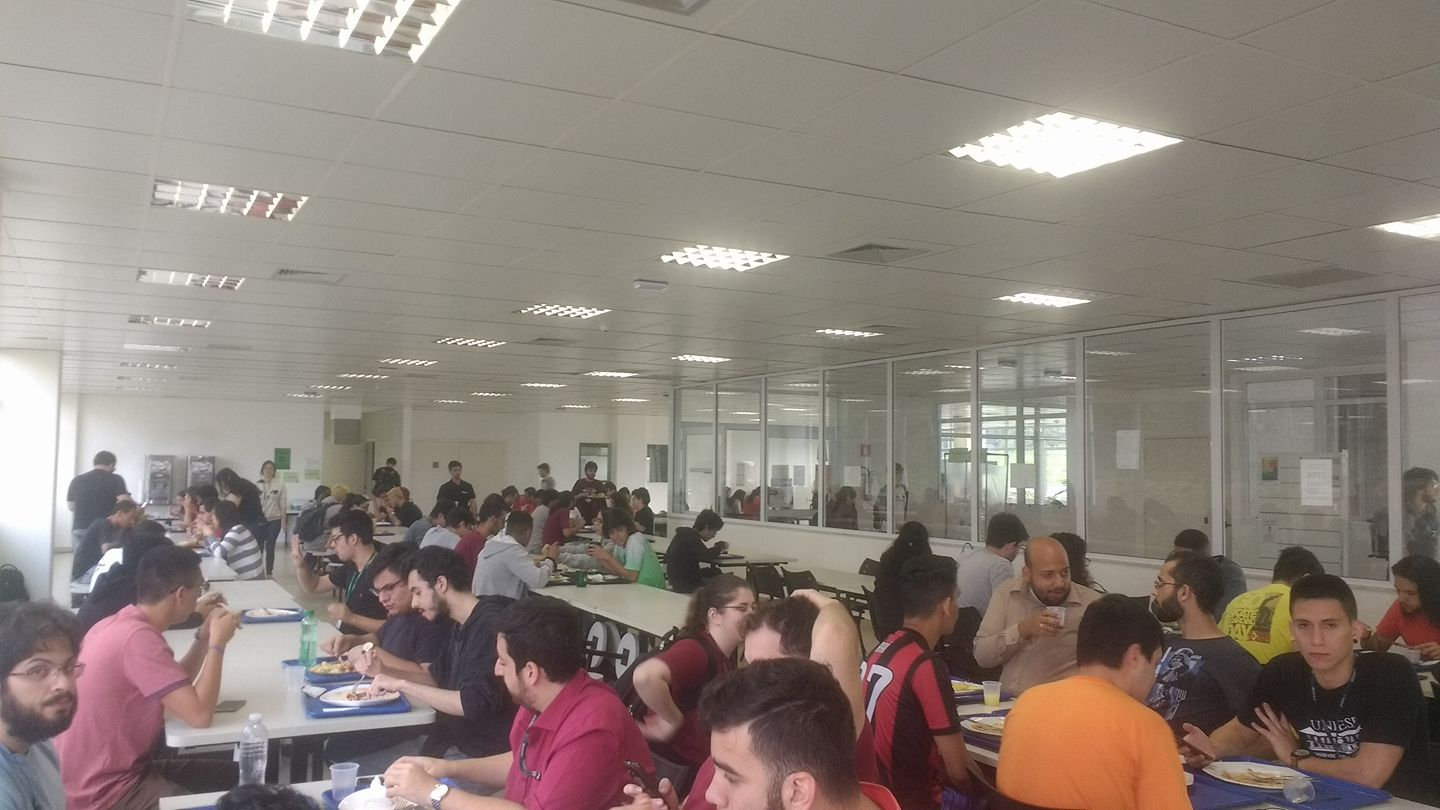
\includegraphics[width=0.7\textwidth]{./Figuras/ru_unifesp.jpg}
        	    \caption{ICT-Unifesp University Refectory}\label{fig:RU_foto}
        	     }
        \end{figure}
    
    \section{Data description}

    This study will make use of two types of data, endogenous and exogenous, which are described below. 
            
    Endogenous data:  are the data of the prediction domain in this case.For this problem, are the daily amounts of meals consumed at lunch and dinner at the University Restaurant (RU) of ICT-Unifesp, quantified daily by the number of students passing the access point, the turnstile.
   Also endogenous data are considered the daily amount of meal tickets sold by the Refectory. In both cases, the information is taken from the class days.  This data are transformed into Neural Networks input, in time series format.
            
    Exogenous data: are all other data outside the prediction domain. For this problem, they are parameters derived from the dates of observations, such as the categorical data representing the day of the week (Monday to Friday), and the climate data.
    
    \section{Data acquisition and treatment}
        The data are obtained from two different sources, the endogenous data being entirely provided through the information technology sector of ICT Unifesp, part of the exogenous data from the date of registration of the endogenous data collected, and the remaining part of the exogenous data, the climate data, are obtained through a weather station closer to ICT Unifesp, located in the city of Taubaté-SP.
        
	    \subsection{Endogenous data} \label{subsec:coleta_endogenos}
        	The historical data of consumption in the restaurant were taken from the current database of subsidized meals at Hospital São Paulo, which manages the data of the cafeterias of all Unifesp units. Only a few authorized employees have access to the institution's database, so to collect such data the present work obtained an authorization with the ICT-Unifesp campus management. Consumption data were only requested for undergraduate students, since the database still contains the consumption information of teachers, graduate students and visitors, but of course with less relevance in quantitative terms. In addition, the consumption pattern of these other strata of the academic environment may influence the process of predicting demands by bringing different trends. In table \ref{table:dadosrestaurante}.
    
        	\begin{table}[!ht]
        	    \centering
        	    \caption{Original format of the original data obtained by the university refectory}
                \rowcolors{2}{gray!25}{white}
                \begin{tabular}{l|l|l}
                    \hline
                    DATE                  & (12/19/2017) & (12/18/2017) \\ \hline
                    BREAKFAST SALES           & 0            & 0            \\
                    LUNCH SALES         & 24           & 71           \\
                    DINNER SALES         & 0            & 0            \\
                    MEAL SALES      & 24           & 71           \\
                    TOTAL SALES          & 24           & 71           \\
                    BREAKFAST ENTRY.            & 0            & 0            \\
                    LUNCH ENTRY          & 42           & 70           \\
                    DINNER ENTRY          & 3            & 24           \\
                    TOTAL ENTRY  MEAL  & 45           & 94           \\
                    TOTAL ENTRANCE         & 45           & 94           \\ \hline
                \end{tabular}
               
                \label{table:dadosrestaurante}
            \end{table}
            
            After the collection, the Refectory's consumption data were transformed in a process of approximation by a temporal series, for an interval of five days, and in each sales record five new attributes were added containing the past values of this same attribute in an interval of five past days. This process adapts the data set to the process of memorizing the entries, structuring the compatible data reading format in the applied Neural Networks models.
            
            The table \ref{table:transformacaodadosrestaurante} exemplifies the new structure of a restaurant data record, with a time interval of five days prior. It is noted that the consumption value of the date 04/20/2017 was removed from the data set, because it is the supervised value to be predicted, since the learning process of neural networks use only data in the past since a previous day.
            
            \begin{table}[!ht]
                \centering
                \rowcolors{2}{gray!25}{white}
                \begin{tabular}{l|l}
                \hline
                    DATE                  & (12/19/2017) \\ \hline
                1 DAY PREVIOUS    & 500        \\
                2 PREVIOUS DAYS & 00                            \\
                3 PREVIOUS DAYS & 300                            \\
                4 PREVIOUS DAYS & 200                            \\
                5 PREVIOUS DAYS & 100                          \\ \hline 
                \end{tabular}
                \caption{Transformation of the refectory records into a time series.}
                \label{table:transformacaodadosrestaurante}
            \end{table}
           
        \subsection{Exogenous data} \label{subsec:coleta_exógenos}
            The exogenous data correlated with consumption are divided into two main types, climate data collected from weather stations near the ICT-Unifesp, and data derived from the dates of consumption records.
    
      	 In terms of the climatic variables used as exogenous data, parameters that may affect the consumption of meals indirectly were considered, such as average ambient temperature, atmospheric pressure, humidity and wind speed. Such parameters can be obtained free of charge by BDMEP - Meteorological Database for Teaching and Research, belonging to the public institution INMET - National Institute of Meteorology, belonging to the Ministry of Agriculture, Livestock and Supply. t is necessary to register in the INMET platform
  \footnote{\url{http://www.inmet.gov.br/portal/index.php?r=bdmep/bdmep}}. The institution contains data registered in digital form since 1961 in the whole country, the historical data referring to periods before 1961 are not yet in digital form and, therefore, are unavailable in BDMEP. It is important to emphasize that the BDMEP takes 90 days to register each new date. 
            	
     	  Besides the environmental data, exogenous data were also generated from the consumption data collected. The date information contained in the indices of the records of endogenous data was derived from various information that represent the consumption behavior in relation to the seasonality of student attendance influenced by the agendas of academic activities.\\
            	The following parameters have been defined:
            	\begin{itemize}
            	    \item Semester 1 or 2 in categorical and binary format;
            	    \item Day of the week in categorical and binary format;
            	    \item Distance in days to previous and subsequent registration;
            	    \item Semester progress in percentage scale;
            	    \item Advance of the month in percentage scale.
            	\end{itemize}
            	
            	The distributed consumption in a five-day window for entry into MLP networks followed a similar pattern with the demand forecasting work in R.U performed by \citeonline{Lopes2008} and \citeonline{Rocha2011}, pictured in Figure \ref{fig:mlp-lopes}. Finally, the Table \ref{table:dataset_final} represents the data set structured and prepared for the process of division into training domains, validation and testing for model training.

       \begin{table}[!ht]
            \centering
            \rowcolors{2}{gray!25}{white}
            \begin{tabular}{c|c|c} \hline
                \multicolumn{3}{c}{ Final structure of the data set indexed by date: } \\
                \hline
                identifier &	variable name					&variable type\\ 
                \hline
                0&	SEMESTER\_1					&int64 \\
                1&	SEMESTER\_2					&int64\\
                2&	MONDAY 						&int64 \\
                3&	TUESDAY 						&int64 \\
                4&	WEDNESDAY						&int64 \\ 
                5&	THURSDAY						&int64 \\ 
                6&	FRIDAY						&int64 \\ 
                7&	DISTANCE\_DAY\_PREVIOUS 	&	int64 \\ 
                8&	DISTANCE\_DAY\_POSTER	&	int64 \\
                9&	PERC\_CONCLUSION\_SEM		&	float64 \\
                10&	PERC\_CONCLUSION\_MONTH		&	float64 \\
                11&	ATMOSPHERIC \_PRESSURE 		&	float64 \\
                12&	TEMPERATURE					&float64 \\ 
                13&	HUMIDITY						&int64 \\
                14&	WIND						&float64\\ 
                15&	SALES\_LUNCH				&int64 \\
                16&	SALES\_LUNCH\_1			&	int64 \\ 
                17&	SALES\_LUNCH\_2			&	int64 \\
                18&	SALES\_LUNCH\_3			&	int64\\ 
                19&	SALES\_LUNCH\_4			&	int64 \\
                20&	SALES\_LUNCH\_5			&	int64 \\ 
                21&	ENTR\_LUNCH				&	int64\\
                22&	ENTR\_LUNCH\_1				&int64 \\
                23&	ENTR\_LUNCH\_2				&int64 \\
                24&	ENTR\_LUNCH\_3				&int64 \\ 
                25&	ENTR\_LUNCH\_4				&int64 \\
                26&	ENTR\_LUNCH\_5				&int64 \\
                27&	ENTR\_DINNER				&	int64 \\ 
                28&	ENTR\_DINNER\_1				&int64\\
                29&	ENTR\_DINNER\_2				&int64 \\ 
                30&	ENTR\_DINNER\_3				&int64 \\ 
                31&	ENTR\_DINNER\_4				&int64 \\
                32&	ENTR\_DINNER\_5				&int64\\
              \hline
            \end{tabular}
            \caption{Final structure of the data set indexed by date
}
            \label{table:dataset_final}
        \end{table}
        Finally, the Table \ref{table:dataset_final} represents the set of data structured and prepared for the process of division into training domains, validation and testing for model training.
        
	\subsection{Pre-processing}
        In the pre-processing stage, the endogenous data is transformed into five-day length time series, normalized with \textit{outliers} removal, and application of scale 0 to 1 so that all the data correspond to the same learning domain. After the completion of these steps, the data set was prepared for the experimental phases 1 and 2, which performed a division of the final data set into distinct time intervals. Although the distribution of the data are presented in dates as a function of time classifying itself in a time series model, it is assumed that their behavior is also impacted by causal relationships with other exogenous variables, such as academic recess, holidays, events, intense rainfall that cause local traffic and impact on the logistics and frequency of the public, among other variables of less apparent causes.
    
        \subsection{Data treatment for model entry}
         	The endogenous data, after structured in the final table of the data sets, goes through the following transformations:
         	\begin{itemize}
                \itemCalculation of the standard deviation of each vector of attributes, and normalization of the maximum values for the ceiling of 3x the standard deviation and minimum of 0; 
                \item	Data transformation in scale of 0 and 1.
            \end{itemize}
            Exogenous data do not be converted into time series, therefore they were treated according to the steps:
            \begin{itemize}
                \item	Data transformation in scale of 0 and 1;
                \item	The categorical binary parameters (days of the week and semester) are already scaled because they are binary categories.
            \end{itemize}
    	\subsection{Experimental Stages} \label{subsec:fases_experimentais}
            The experimental process was carried out in two distinct routes of division of the temporal domain of the data set, and the results obtained between the two phases were compared.
            
            The data set covering the period 2017 to 2019 was divided into a training, validation and testing set as follows: 
            
            \paragraph{1st Phase with validation in the 1st semester of 2018 and test in the 1st semester of 2019}
                 In this script, the validation semester that makes up the data set for  \textit{backpropagation} training of neural networks contemplates the first semester of 2018 and the test set contemplates the first semester of 2019.
                Data from 2017 contemplating the 1st and 2nd semesters, and 2018 contemplating the 2nd semester, were used for training. The results obtained in this division were used to validate the hypothesis that the models specifically learn the seasonality of consumption in the first semester, doing better in the tests carried out in the first semester of 2019, compared to the other trained models with validation throughout the year 2018.
                Therefore, the data set of the first phase includes the following domain:
            \begin{itemize}
                    \item Model training set, contemplating the first and second half of 2017 and second half of 2018;
                    \item Validation set of the models, contemplating the first half of 2018;
                    \item Test set of models, contemplating the first half of 2019.             
            \end{itemize}
            
            \paragraph{2nd phase with training in 2017, validation in 2018 and test in 2019}
                In this phase, the sets were divided according to their description and the best model found goes through a final test phase in the domain of the first phase (test only in the first half of 2019).
                The metrics obtained in this test were compared with the best model of the first phase.
    
    \section{Model definition and training}
            %\paragraph*{Sobre a necessidade de implementar modelos mistos}
                In the data set of this work, the data obtained are divided into temporal and endogenous data (such that each record of consumption and sale brings the information of its domain in a time interval of five days prior) and discrete and exogenous data, being categorical date variables for each record and climate variables.
                
                Therefore it was necessary to implement specific models for time entries and specific models for discrete entries.
                For the final output a committee of endogenous and exogenous Neural Networks was implemented, with a perceptron neuron at the output, receiving the two values of the endogenous and exogenous models for the regression of the outputs of the two networks to the value that will be the prediction of consumption.
         	\paragraph{Endogenous models}
         	\begin{itemize}
                \item	Development of low depth perceptron networks to evaluate network learnability;
                \item	Increase network depth and evaluate changes in RMSE loss function; 
                \item	Implementation and evaluation of models with GRU recurring networks, as shown in Figure \ref{fig:gru-arch} that are specially developed for learning with data memorization, and in the case of this work, can memorize the weekly seasonality of consumption (in a five-day interval).
            \end{itemize}
            \paragraph{Mixed Models : Endogenous and Exogenous}
                \begin{itemize}
                    \item For the time data (consumption and sales) we used the best endogenous models from previous experiments for endogenous inputs.
                    \item For the discrete and categorical data the input of this data was adapted to perceptron network
                    \item  The exit of the two Neural Networks was concentrated in a perceptron, creating a committee of Neural Networks to obtain the expected final exit.
                \end{itemize}
            
	\subsection{Hyper parameters : Activation and optimizer function}
        As based on the Chapter \ref{cap:teoria} in section \ref{sec: perceptron} the activation function gives perceptron the ability, when connected to a network, to solve linear and non-linear problems, adding adaptation and improvisation when solving programs that are not contained in its power data.
        So for the hidden layers of the developed MLP neural networks the ReLu function will be applied and for the output neuron the linear function will be applied, and the training optimizer performs the function of optimizing the convergence time of the readjustment of the weights to the ideal values, being chosen the ADAM optimizer with learning rate set at 0.001.

    \section{Test and Evaluation Metrics}
       The main metrics for the evaluation of the models are the \textit{Root Mean Squared Error} (RMSE), The Pearson correlation coefficient (R), and the ''chi-square coefficient'' defined as $R^2$. These statistical metrics were used in the test steps to evaluate the proximity of the model predictions to the actual consumption behavior. The equations \ref{eq:RMSE} and \ref{eq:Pearson} present the formulation for the RMSE and the Pearson coefficient (R), respectively.
       
       \begin{equation}
           RMSE = \sqrt{\frac{1}{n}  \sum_{i=1}^n (x_i^{est} - x_i^{obs})^2}
           \label{eq:RMSE}
       \end{equation}
       
       \begin{equation}
           R = \frac{\frac{1}{n}  \sum_{i=1}^n (x_{est} - \bar{x}_{est}) * (x_{obs} - \bar{x}_{obs})}{\sigma_{est} * \sigma_{obs} }
           \label{eq:Pearson}
       \end{equation}
       
       Where "est" are the estimated values; "obs" are the actual values; n is the number of samples ; $\sigma$  is the default deviation; R is the linear correlation; $\bar{x}$ is the mean of x. We also evaluated the positive and negative errors between the predicted and real values, to represent how many meals would be discarded and how many would be missing if meal production were according to the model predictions.
       
  % ----------------------------------------------------------
  % \chapter{METODOLOGIA}
  % ----------------------------------------------------------